\documentclass[conference]{IEEEtran}
\IEEEoverridecommandlockouts
% The preceding line is only needed to identify funding in the first footnote. If that is unneeded, please comment it out.
\usepackage{cite}
\usepackage{amsmath,amssymb,amsfonts}
\usepackage{algorithmic}
\usepackage{graphicx}
\usepackage[percent]{overpic}
\usepackage{textcomp}
\usepackage{xcolor}
\usepackage{comment}
\usepackage{caption}
\usepackage{subcaption}
\usepackage{graphicx}
\usepackage{nicematrix}

\usepackage[colorlinks=true, linkcolor=blue, citecolor=blue, urlcolor=blue]{hyperref}
%%%%%%%%%%%%%%%%%%%%%%%%%%%%%%%%%%%%%%%%%%%
\setlength{\textfloatsep}{5pt plus 1pt minus 1pt}  % space after top/bottom floats
\setlength{\intextsep}{5pt plus 1pt minus 1pt}     % space around in-text floats
%%%%%%%%%%%%%%%%%%%%%%%%%%%%%%%%%%%%%%%%%%%

\def\BibTeX{{\rm B\kern-.05em{\sc i\kern-.025em b}\kern-.08em
    T\kern-.1667em\lower.7ex\hbox{E}\kern-.125emX}}
    
\begin{document}

\title{Multiple nutrient sensing for smart agriculture}

\makeatletter
\newcommand{\linebreakand}{%
  \end{@IEEEauthorhalign}
  \hfill\mbox{}\par
  \mbox{}\hfill\begin{@IEEEauthorhalign}
}
\makeatother

\author{\IEEEauthorblockN{John White}
\IEEEauthorblockA{\textit{School of Engineering Mathematics and Technology} \\
\textit{University of Bristol}\\
Bristol, England \\
aa22951@bristol.ac.uk}
\and
\IEEEauthorblockN{Thomas Wilson}
\IEEEauthorblockA{\textit{School of Engineering Mathematics and Technology} \\
\textit{University of Bristol}\\
Bristol, England \\
fj23813@bristol.ac.uk}
\linebreakand %
\IEEEauthorblockN{Raj Dhakan}
\IEEEauthorblockA{\textit{School of Engineering Mathematics and Technology} \\
\textit{University of Bristol}\\
Bristol, England \\
xn23972@bristol.ac.uk}
\and
\IEEEauthorblockN{Ross Duncan}
\IEEEauthorblockA{\textit{School of Engineering Mathematics and Technology} \\
\textit{University of Bristol}\\
Bristol, England \\
lw23535@bristol.ac.uk}
}
\maketitle

\begin{abstract}
NIR Spectroscopy (NIRS) is an established method used for predicting properties of plant matter. In potato agriculture, spectroscopy provides the potential to predict nutrient levels in plants efficiently, leading to quicker and more accurate treatment responses. Supervised multivariate regression models can be used in this setting to predict multiple nutrients simultaneously based on samples with NIRS reflectance and chemical measurement data. Such datasets normally have high dimensionality and small sample size. This study finds that preprocessing NIRS readings through baseline correction and extracting peaks for features can improve the performance of Multi Linear Regression (MLR) and Random Forest models (and depending on whether the samples are dried or fresh), while having a nominal to detrimental affect on PLS Regression. Multi Task Lasso and Elastic Net were also compared along with these to a MLR baseline, but optimised with minimal regularisation penalty using the preprocessed data. Overall, Random Forest performed the best based on $R^2$ and RMSE metrics for both dried ($R^2$=0.423, RMSE=0.0836) and fresh ($R^2$=0.025, RMSE=0.1027) samples.
\end{abstract}

\section{Introduction}
Near-Infrared spectroscopy (NIRS) is a technology used in 'precision agriculture' \cite{Cavaco2022}, classified as a remote sensing technique \cite{Jafarbiglu2022}, which can produce data to help maintain optimal nutrient levels in potato plants \cite{Abukmeil2022}. Using the reflectivity readings of leaf samples produced by NIRS (as features) together with measurements of nutrients (as targets), supervised machine learning (ML) techniques can be used to predict plant nutrient levels faster, more efficiently and cost-effectively when compared to traditional laboratory tests. NIRS produces high-dimensional reflectivity readings characterised by $p \gg n$ (with $p$ features and $n$ samples), and there are multiple nutrients of interest in the health/yield of potato plants. The purpose of this study is to extend the research of Abukmeil et al. \cite{Abukmeil2022}, which focused on the effectiveness of using floral spectroscopy to predict plant nutrient concentrations using a Lasso multi-linear regression (MLR) approach, to:
\begin{itemize}
    \item Analyse the effect of data preprocessing methods on spectral data and on predictive performance.
    \item Establish the impact of the elected data processing strategy and its suitability against multivariate models commonly used in similar settings.
\end{itemize}
Initially, the data is parsed through a preprocessing pipeline featuring baseline correction of a dataset and extracting the features of interest, which is compiled over multiple seasons to maximise generalisation. A univariate MLR baseline is used to assess the performance of basic data reduction techniques such as binning and Principle Component Analysis (PCA), along with more tailored techniques of baseline correction coupled with peak feature extraction. The resulting pipeline was compared to the performance of a multivariate application of a Partial Least Squares Regression (PLS or PLSR) model, Multi Task Lasso (MTL), Multi Task Elastic Net (MTEN) and Random Forest (RF) models. The effectiveness of the pipeline for fresh and dried sample modes is examined separately, as they present different reflective signals.

\section{Literature Review}

\subsection{Problem Domain}
Precision agriculture is an evolution in agricultural practices that uses technology to improve productivity, efficiency \cite{GAO-24-105962}, and sustainability \cite{Bongiovanni2004}. The growth in diverse and accessible sensing technologies provides the opportunity to use data to help predict conditions and respond to them with more automated and precise feedback into the agricultural process \cite{Herrmann2021}. Among these sensing technologies is the measurement of plant sample reflectivity over different light wavelengths for various applications, including measuring contaminants, assessing plant quality and nutrient levels \cite{Workman2024}. Micro and macro nutrient balance in potato plants directly and indirectly impacts tuber quality and yield \cite{Oivukkamaeki2023}. Naumann et al. \cite{Naumann2020} address the impacts of macronutrients and the complex nature of the relationships between them on quality and yield, and Koch et al. \cite{Koch2020} illustrate that the importance of balance, the 'law of the minimum' and the nature of a saturation curve, where no further benefit to plant development can be realised, or impairment to quality can occur. Such evidence stresses the importance of accuracy when assessing nutrient levels in plants and any supplementary response. The use of spectroscopic reflectivity readings as independent variables for the concentrations of nutrients in plants is not new. The first studies of NIRS on plant tissue began in the mid-1970s \cite{Prananto2020} and have since shown promise under the later umbrella of precision agriculture as a means of maintaining optimal nutrient balance. 

\subsection{Review of Methods}\label{lit_review_methods}
Different ML models have been experimented with for their efficacy in predicting nutrient concentrations in soil and plant material. Waegeman et al. \cite{waegeman2018multitargetpredictionunifyingview} propose the family of multivariate regression techniques for settings where multiple dependent variables are sought. PLSR has become a popular method in chemometrics \cite{Liu2015, HaibinLiao2012} and is related to methods like Principal Component Regression (PCR) and Ridge Regression, unified by an approach termed Continuum Regression \cite{Rosipal2006}. PLS-2 regresses multiple response variables and finds a set of latent variables that explain the covariance between independent and dependent variables simultaneously \cite{Garson2016, Liu2022}. Such methods minimise the "curse of dimensionality" using inherent dimensionality reduction (DR) or regularisation processes. While PLSR does not use explicit regularisation (more implicit as part of its DR), Lasso Regression is a formal regularisation algorithm that offers multivariate \cite{Rauschenberger2021}, or further, multi-task methods \cite{Obozinski2006}. An extension that combines both Lasso and Ridge Regression is ElasticNet that has been found to provide better interpretability over PLSR \cite{Fu2019}, and can overcome limitations of some regression models that are less successful in settings with high multicollinearity and propensity to over-fitting \cite{Liu2024}. Regression methods that can find non-linear relationships and are evidenced as giving positive results in similar settings include Gaussian Process Regression \cite{Rasmussen2006,Chen2007}, Support Vector Regression \cite{Tange2015, Fearer2022} and Deep Learning \cite{Cui2018, Huang2023}. Ensemble methods such as Random Forest \cite{Nawar2017, Fearer2022} and Gradient Boosting \cite{Zheng2024, Nawar2017} have also been the subject of recent research with NIRS prediction settings. Research suggests the use of stacked regression (capable of combining the strengths of different models) shows encouraging results over single-method approaches \cite{Dumancas2022}.
\section{Dataset}\label{Dataset}
The data in this study consist of NIRS reflectance readings (features) and 14 (macro and micro) nutrient concentrations (targets), where concentration is either measured in parts per million (PPM) or percentage (PCT) as described by the matrix in Table \ref{tab:desc_nutrients}. Reflectance is measured over a spectrum of wavelengths between 400nm-2500nm at either 0.5nm or 1nm intervals. The sample size $n=674$ (excluding null records) can have features $p=4200$ (at the higher resolution of 0.5nm), defining the dataset as high-dimensionality low-sampling size (HDLSS). The data is further categorised by its season (of which there are 4) and the two sampling modes (fresh and dried). Fig. \ref{fig:distr_viol} shows the distribution of all targets (\texttt{MinMax} scaled) in season 1, split into the two sampling modes. 

\begin{figure*}
    \centering
    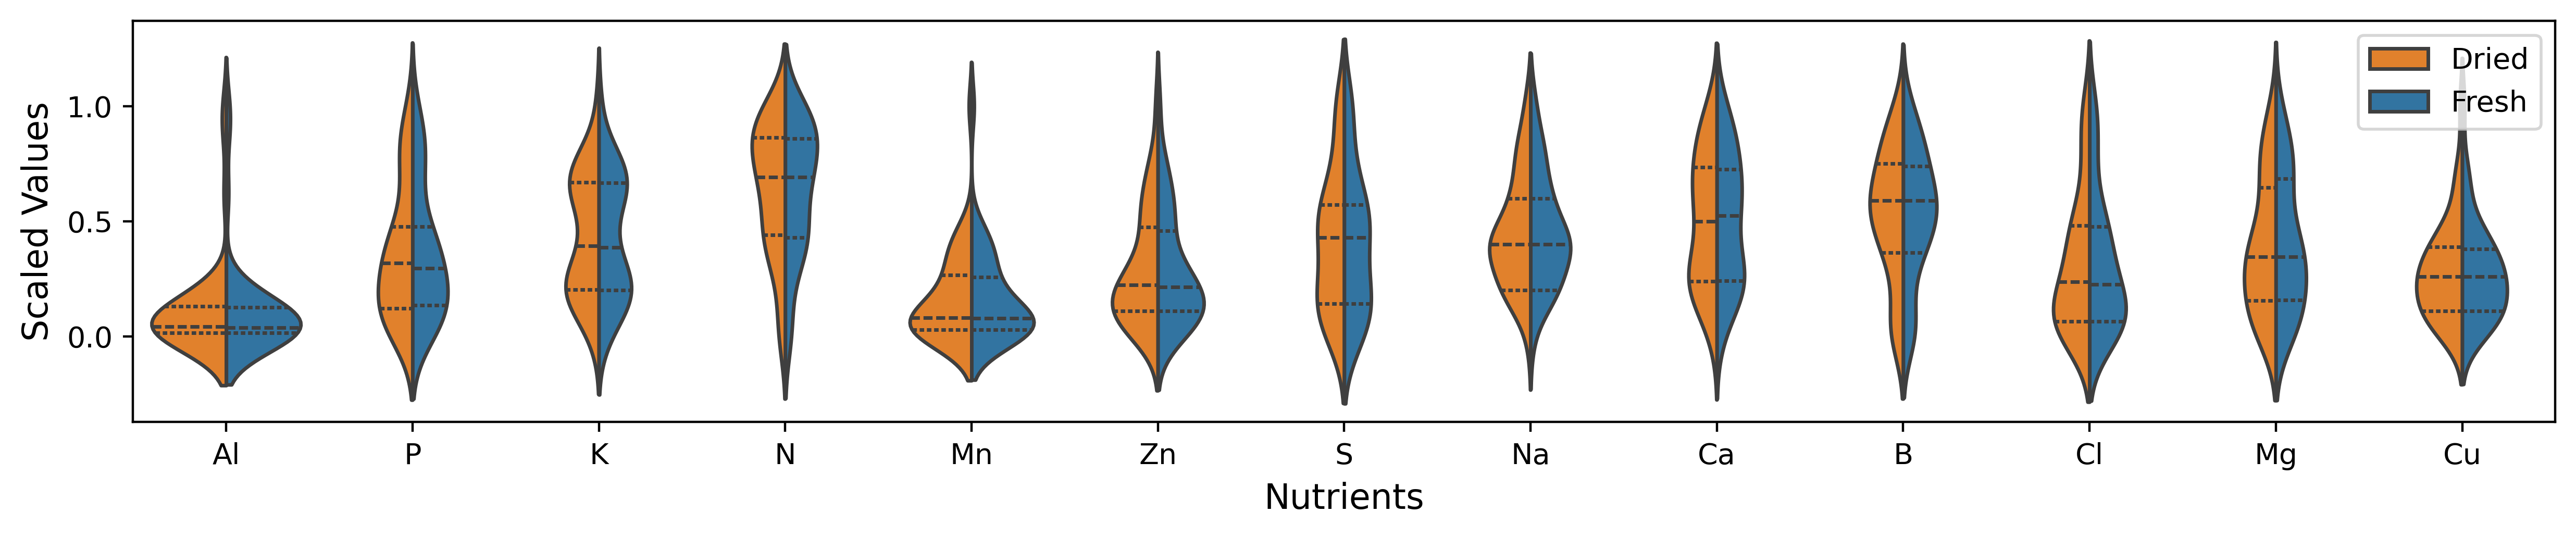
\includegraphics[width=1\linewidth]{Figures/distr_viol_plot.png}
    \caption{Distribution of nutrient concentrations in season 1.}
    \label{fig:distr_viol}
\end{figure*}

The graph in Fig. 1 shows that the distribution is not normal but is generally highly (positively) skewed, with some exceptions showing bimodality. In addition, when the same nutrient is compared to itself across different seasons, the distribution is dissimilar. Moreover, the distribution is identical between the two sample modes, which can be explained through the principle of mass conservation, whereby the concentration of nutrients is preserved after the petiole sample is dried. Another key finding is that the targets are correlated. Although some pairwise combinations of targets are consistently highly correlated regardless of the season, some are inconsistent. Both of these observations are evidenced by a small subset of pairwise nutrient combinations in Fig. \ref{fig:corr_vals}. Finally, Fig. \ref{fig:peak-stages}a shows the variations in the reflectance values between samples across the spectrum used for ML.

\begin{figure}[b]
    \centering
    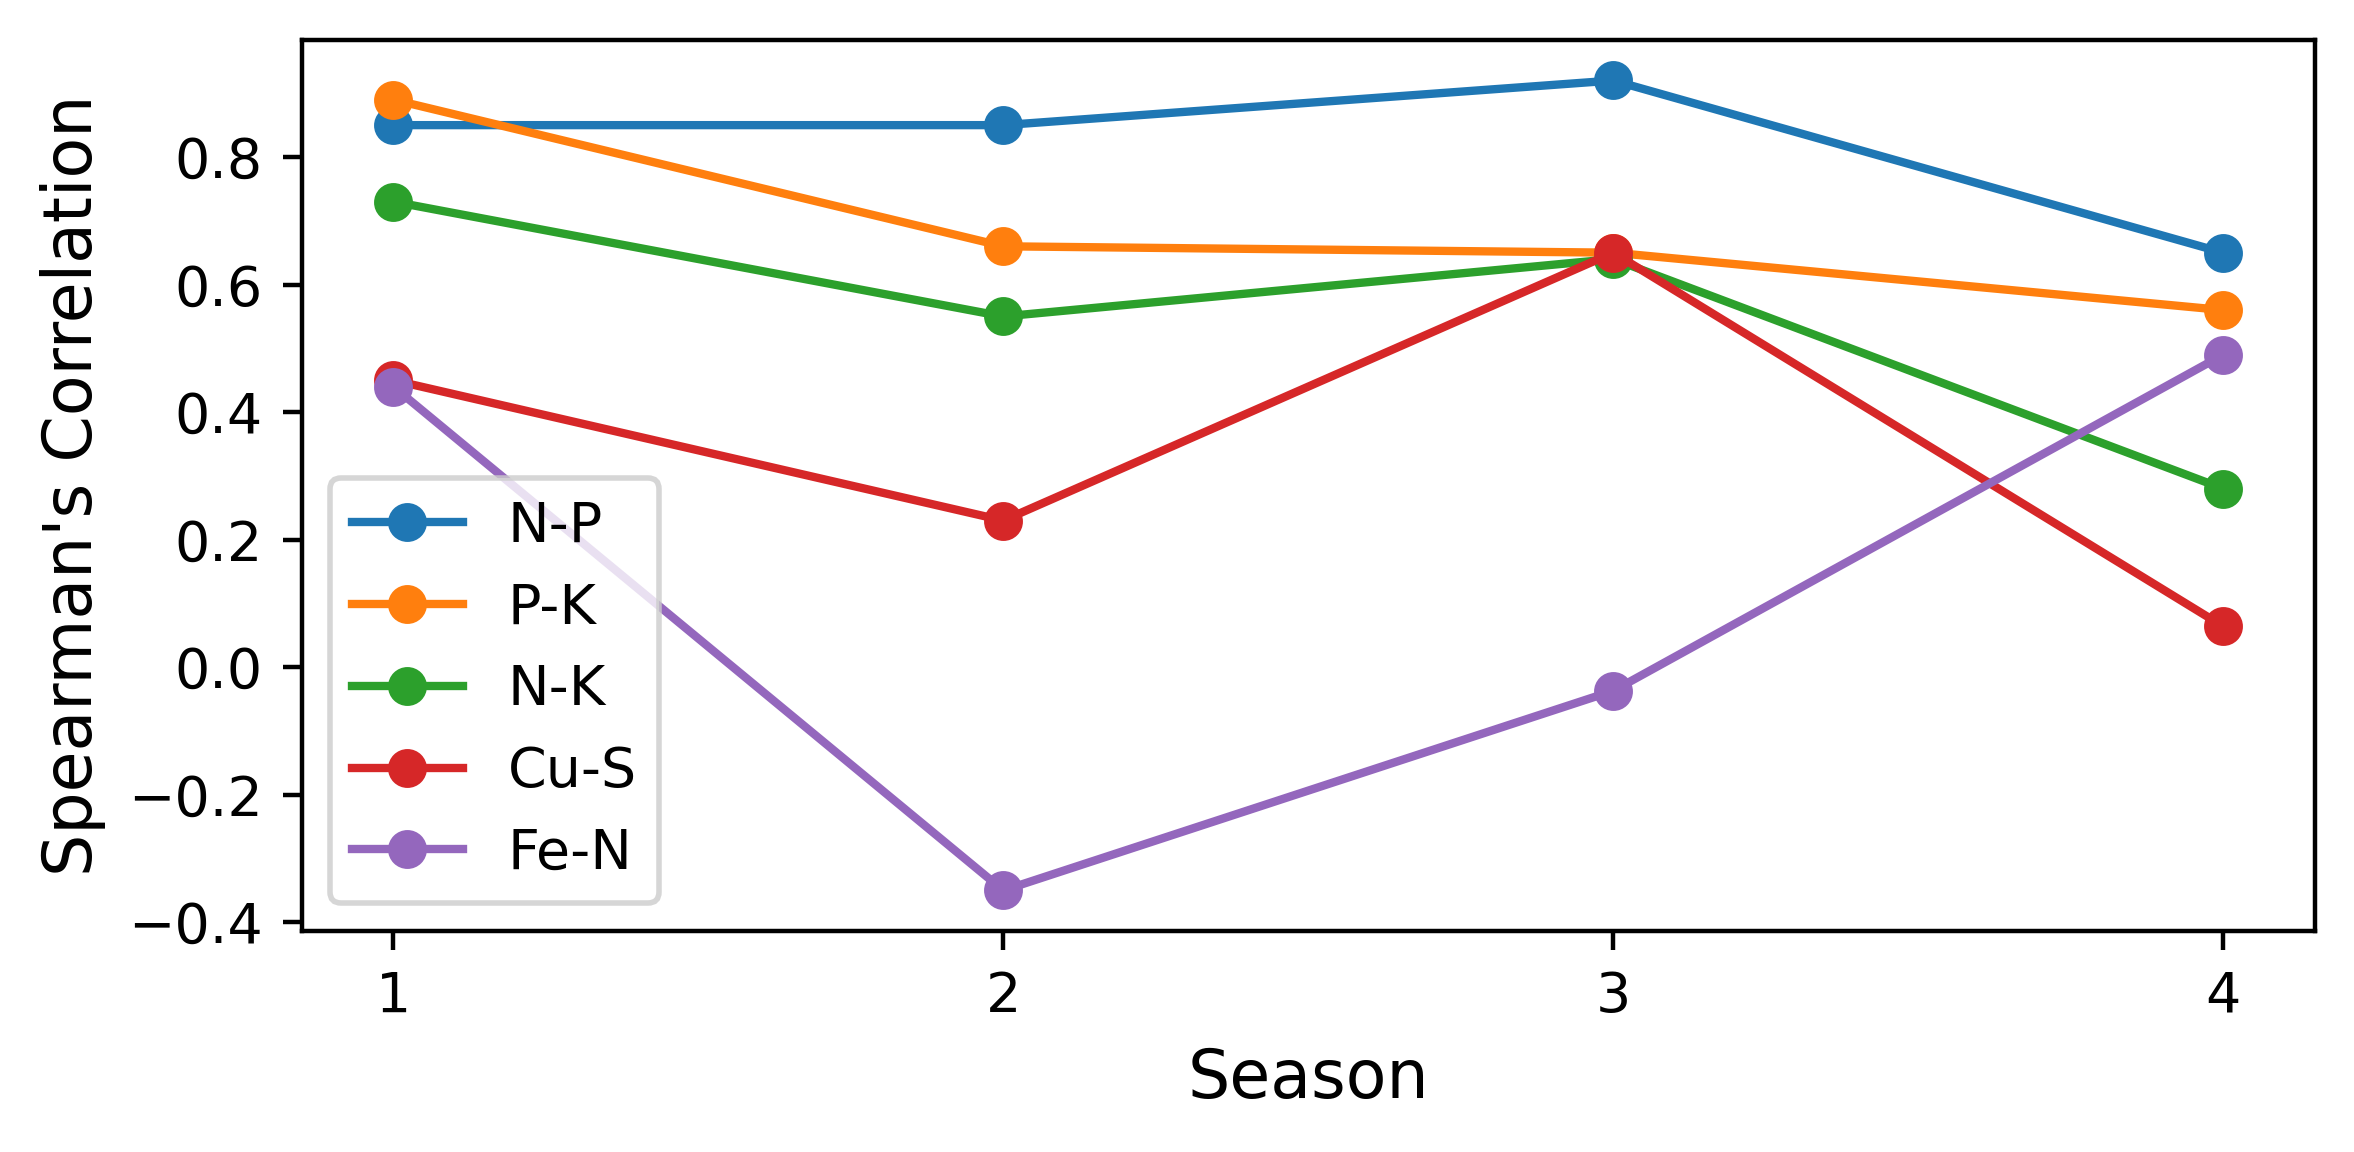
\includegraphics[width=1\linewidth]{Figures/corr_vals.png}
    \caption{Spearman's correlation across seasons.}
    \label{fig:corr_vals}
\end{figure}

\begin{table}
    \caption{Description of nutrients.}
    \centering
    \begin{tabular}{|c|c|c|}\hline
         & \textbf{Macro} & \textbf{Micro} \\\hline
        \textbf{PPM} & - & Al, B, Cu, Fe, Mn, Zn\\\hline
        \textbf{PCT} & Ca, Mg, N, P, K, S  & Cl, Na \\\hline
    \end{tabular}
    \label{tab:desc_nutrients}
\end{table}

\section{Methodology}

\subsection{Data Partitioning}\label{DP}
Given the data is HDLSS, a stratified test-train split (of 20:80) was implemented to maximise the training data, where stratification occurs on the season for each sampling mode, resulting in separate train-test datasets and ML models for each. This allows for a proportional representation of each season to account for the fact that targets in each season have a dissimilar distribution. By preserving the same ratios in the test set, it is ensured that no one season is over-represented due to an unbalanced number of samples from each, which may form biased ML models.

\subsection{Multivariate Regression}\label{Models}
Given the targets are not only related to the features but also intercorrelated, this setting demands the prediction of multiple targets simultaneously (multi-target prediction - MTP) over a continuous feature set, characterised as Multivariate Regression (MVR). As formally described by Waegman et al. \cite{waegeman2018multitargetpredictionunifyingview}, where instances of $x \in \mathcal{X}$ and targets $t \in \mathcal{T}$, the training set $\mathcal{D}$ is a set of $(\mathbf{x}_i, \mathbf{t}_j, y_{ij})$ where $y_{ij} \in \mathcal{Y}$ is a score that represents the relationship between $\mathbf{x}_i$ and $\mathbf{t}_j$. $\mathcal{Y}$ is a vector of real-number scores, which can be arranged in an $n \times m$ matrix ($\mathbf{Y}$), where $n$ are the instances and $m$ are targets. The aim of MTP and thus its subclass MVR is to predict the scores ($\mathcal{Y} = \mathbb{R}$) for permutations $(\mathbf{x}, \mathbf{t}) \in \mathcal{X} \times \mathcal{T}$. To conduct MVR, the below models were implemented in the study using Python's Scikit-Learn Library:
\begin{enumerate}
    \item \textbf{MLR} is adopted as a baseline for univariate analysis. The implementation used in the study fits a separate regression model for each target whilst making use of all features. Each model learns a distinct set of coefficients tailored to its specific target. As this approach treats targets independently, it does not capture interdependencies between them. This makes it a useful baseline for quantifying the added value of more complex multivariate models considered in this study.
    \item \textbf{PLSR} is a cross-decomposition algorithm that extracts components that best explain the shared variance between data sets $\textbf{X}$ and $\textbf{Y}$. PLSR derives orthogonal components from $X$ that capture the covariance between $X,Y$, converting the correlated variables into a set of uncorrelated components. This underlines its strength in handling high multicollinearity. Although related, it differs from PCA in that instead of maximising variance in $X$, it maximises covariance in $X,Y$. By eliminating multicollinearity, it prevents overfitting by reducing the bias of highly correlated variables, while finding linear combinations of the $X$ variables that have high correlation with $Y$.
    \item \textbf{RF} is an ensemble machine learning method, combining predictions from multiple individual decision trees (hence 'forest'). Multiple subsets of data are selected using the bootstrapping method, with which decision trees are trained on. Regularisation can be set by determining the maximum depth of trees, the minimum number of samples required to split a node, and the minimum required in a leaf node.
    \item \textbf{MTL} uses $L_1$ regularisation, which reduces dimensions by forcing some coefficients to zero \cite{Zou2005}, allowing for the selection of the same subset of features across all tasks. The strength of this regularisation is dictated by the $\lambda$ term - the larger the term, the greater the regularisation \cite{Abukmeil2022}.  
    \item \textbf{MTEN} incorporates both $L_1$ and $L_2$ regularisation, which is effective in the $p\gg n$ case where features may be strongly correlated \cite{Zou2005}. $L_2$ (Ridge) regularisation uses a penalty term for the loss function, which may reduce coefficients minimising the impact of multicollinearity where it may exist. Both reduce over-fitting by removing noise and multicollinearity by balancing $L_1$ and $L_2$ regularisation on regression coefficients. MTEN and MTL are designed with the intention of multi-task learning but can be applied to multi-target prediction, by utilising a joint regularisation term to encourage feature selection relevant to multiple outputs.
\end{enumerate}

\subsection{Model Evaluation}\label{Model Evaluation}
To evaluate and compare model performance, the characteristics of the targets must be considered first. Since the targets are measured in different units and also have different ranges within the same units, the values are scaled. Section \ref{target_scaling} outlines how target scaling avoids the need for normalised error metrics at the point of evaluation. 

The two metrics used for evaluating the models are:
\begin{enumerate}
    \item Root Mean Square Error (RMSE) is the square root of the Mean Squared Error (MSE), and provides an error measure in the same units as the variable being predicted \cite{plevris2022investigation}. The benefits for MVR are that it gives better interpretability across all targets, it's a more intuitive scale and focuses on magnitude. Given that it is derived from the MSE, it is sensitive to outliers \cite{plevris2022investigation}, though less so, given that large values will carry less weight in measurement. It is defined as \cite{plevris2022investigation}:
\begin{equation}
    RMSE = \sqrt{\frac{\sum(y-\hat{y})^2}{n}} \label{eq1}
\end{equation}
    \item Coefficient of Determination ($R^2$) is the proportion of variation in the target that is predicted from the input and is a measure of how well observed outcomes are predicted by a model \cite{plevris2022investigation}. $R^2$ provides values in a consistent range [0,1], with larger values implying a more successful model, thus more intuitive for comparison. It is defined as \cite{plevris2022investigation}:
\end{enumerate}
\begin{equation}
    R^2 = 1- \frac{\sum(y-\hat{y})^2}{\sum(y-\overline{y})^2} \label{eq2}
\end{equation}  

To evaluate the effectiveness of each preprocessing step and also for tuning hyperparameters of models, the above metrics were used along with the cross validation method. Particularly for model tuning, SciKit Learn's \texttt{GridSearchCV} was adopted, using a consistent 5-fold approach over the training set, taking the average performance of prediction scores against each fold, for each permutation of hyperparameters. The most performant permutation of hyperparameters was selected based on the minimal loss over those tested. RMSE (of scaled targets) was the metric used as the loss measure.

\subsection{Preprocessing}\label{PP}
\subsubsection{Imputation}\label{Imputation}
Of the 14 nutrients, Cl was omitted as more than 90\% of the samples, throughout the dataset, were null. Regarding the feature set, there are also missing values due to the discrepancies in the resolution (0.5nm and 1nm) between seasons. Therefore, imputation of missing values was crucial to maximise the number of usable samples. 

The data was imputed separately on training and test data to avoid data leakage. Missing nutrients were imputed using K-Nearest Neighbour (KNN) model as it preserves the multivariate structure, but also because it is non-parametric. To impute the missing 0.5nm values for seasons with a lower resolution of 1nm, linear interpolation was implemented because of its simplicity in approximation for a small wavelength range.
\vspace{0.1cm}
\subsubsection{Outlier Removal}
Outliers can be naturally occurring extreme values or anomalies resulting from human/machine error that distort the underlying data patterns. Removing only true anomalies is important, as preserving the naturally extreme values allows the ML model to link feature ranges to extreme target values. Four possibilities were evaluated using cross-validation scores:
\begin{itemize}
    \item \textbf{No outlier removal}.
    \item Outlier removal in \textbf{targets only}: this assumes human error when calculating the concentration of petiole samples in the laboratory. Here, the Isolation Forest algorithm was used, given that it is non-parametric, can handle multi-dimensional data with no preprocessing and is specifically designed for outlier detection \cite{Liu2012}.
    \item Outlier removal in \textbf{features only}: this assumes machine error when collecting reflectance data. The feature set is first reduced to two principal components for each sample using PCA. Based on the centres of each season cluster, any data points residing past the 95th percentile distance from the centre are classed as an outlier.
    \item Outlier removal using \textbf{both targets and features}: this assumes that true anomalies are the non-overlapping outlier sample records from targets only and features only analysis. Any sample records that match across both sets are assumed to be natural extreme values.
\end{itemize}
The outlier removal implementation was done only on the training set, as it was hypothesised that it would make the learning data cleaner. Cross-validation results showed that not removing any outliers produced better results across all ML models tested in the study.

\subsubsection{Baseline Correction}
Baseline correction is a preprocessing step in spectroscopy to remove unwanted background variations that can obscure important spectral features. Prior studies have demonstrated that effective baseline correction significantly improves the interpretability and predictive performance of models built on spectral data \cite{Li2024, FengZhang2020, Eilers2005}. Unwanted variations in the baseline may arise from several sources. Instrumental drift causes gradual changes in the spectrometer’s response over time. Scattering effects, especially common in NIR and Raman spectroscopy, occur when the sample's morphology influences the reflectance. Another contributor is fluorescence, where broad overlapping emission signals can obscure genuine absorption features. Lastly, environmental factors such as changes in temperature, humidity, and other measurement conditions during acquisition can also lead to baseline fluctuations. 

These effects introduce smooth, large-scale trends in the spectra, which can dominate and obscure the fine, sharp absorption features linked to material composition.

Fig. \ref{fig:peak-stages}a shows some of the sample spectra and it is observed that the reflectance spectra for all samples follow a similar general shape dominated by these smooth baseline variations. This similarity between samples is unhelpful for ML models, which rely on capturing differences between samples to make accurate predictions. The following assumptions have influenced the chosen baseline correction method. First, smooth variations across wavelengths are primarily interpreted as background noise, as previously described. Second, sharp localized troughs in reflectance (corresponding to increases in absorbance) are taken to indicate the presence of target elements. Finally, differences in the amplitudes of reflectance in these regions are considered meaningful for modelling element abundances. 
\begin{figure}[htbp]
  \centering

  % ---------- (a) ----------
  \begin{subfigure}{0.5\textwidth}
    \centering
    \begin{overpic}[width=\linewidth]{Figures/Reflectance Spectra.png}
      \put(10,34){\textbf{(a)}} % 3 % from left, 90 % from bottom
    \end{overpic}
  \end{subfigure}

  \vspace{-0.61cm}

  % % ---------- (b) ----------
  % \begin{subfigure}{0.5\textwidth}
  %   \centering
  %   \begin{overpic}[width=\linewidth]{Figures/Absorbsion Spectra.png}
  %     \put(10,30){\textbf{(b)}}
  %   \end{overpic}
  % \end{subfigure}

  % \vspace{-0.61cm}

  % ---------- (c) ----------
  \begin{subfigure}{0.5\textwidth}
    \centering
    \begin{overpic}[width=\linewidth]{Figures/ALS corrected spectra with Lines.png}
      \put(10,34){\textbf{(b)}}
    \end{overpic}
  \end{subfigure}

  \caption{Application of baseline correction: (a) raw reflectance spectra, (b) absorbance spectra after \(\log(1/R)\) transformation followed by ALS using parameters $\lambda=10^{5}$, $p=0.01$, with key wavelengths highlighted.}
  \label{fig:peak-stages}
\end{figure}

In Fig. \ref{fig:peak-stages}a, a transformation of $A = log(1/R)$ is applied, commonly this is found to improve results in similar studies as it is thought to convert the non-linear reflectance measurements into linear absorbance measurements \cite{min2005determination}.
  
Given these assumptions, Asymmetric Least Squares (ALS) baseline correction is the chosen method and a common choice for chemometric analysis \cite{FengZhang2020}. ALS is particularly well-suited for the requirements because it penalises deviations above the baseline more heavily than below and preserves sharp absorption features in the spectra while smoothing broader baseline trends.

ALS solves the following optimisation problem:

\begin{equation}
\min_{z} \left( \sum_{i=1}^{n} w_i (y_i - z_i)^2 + \lambda \sum_{i=2}^{n-1} (z_{i-1} - 2z_i + z_{i+1})^2 \right) \label{eq3}
\end{equation}


where:
\begin{itemize}
    \item \( y_i \) is the observed absorbance at wavelength index \( i \),
    \item \( z_i \) is the estimated baseline,
    \item \( w_i \) is a weight controlling the influence of each point,
    \item \( \lambda \) controls the smoothness of the baseline.
\end{itemize}

The weights \( w_i \) are updated iteratively as:
\begin{equation}
w_i = 
\begin{cases}
p, & \text{if } y_i > z_i \quad \text{(peak region)} \\
1 - p, & \text{if } y_i \leq z_i \quad \text{(background region)}
\end{cases} \label{eq4}
\end{equation}
where \( p \in (0, 0.5) \) controls the asymmetry between peaks and background points; the smaller the value the more asymmetric  the baseline.

\vspace{0.1cm}
  
The resulting spectra after applying ALS in Fig. \ref{fig:peak-stages}b has been flattened to an identical level, at an absorbance level of approximately 0.16 across all samples. The rest reveals clear sharp peaks which occur for the same wavelength across samples but with different amplitudes.
\subsubsection{Dimensionality Reduction (DR)}
Due to the low sample count combined with high dimensionality and multicollinearity, any model would have a high risk of introducing noise and over-fitting. It would also significantly increase model complexity and slow down training. DR methods solve these issues and, depending on the model used, also help with interpretability. Various DR methods were applied to features when tuning the data pre-processing pipeline:
\begin{itemize}
    \item \textbf{Binning} reduces the number of features by taking the mean of the reflectance values over the specified wavelength range.
    \item \textbf{PCA} handles the multicollinearity between features by reducing them to few uncorrelated principle components.
    \item \textbf{Peak Feature Extraction} leverages the peaks identified in Fig. \ref{fig:peak-stages}b following baseline correction, for each sufficiently prominent peak, the minimum amplitude, maximum amplitude, and area under the curve were extracted. These extracted values serve as the features used as inputs for subsequent machine learning models.
\end{itemize}
Analysing binning shows a pattern of accelerated degradation in performance past an averaging over 4nm. Both sample modes show peaks of poor performance at dried (bin size of 8) and fresh (bin size of 11), after which the validation performance starts to reduce asymptotically to a lower RMSE score, a concerning phenomenon as it is clear at some point important information may be lost. This implies the need for a less crude method to reduce noise in the data.

During cross-validation, PCA provided no easily discernible optimal number of components. Given the small sample size, the maximum number of components for dried and fresh were 77 and 58, respectively. Scree plots determined that the first two components explain the majority of variance for both dried and fresh samples. Likely losing finer details or subtle patterns in the data, PCA was omitted as a data-reduction method in the absence of more in-depth investigation. Although PCA produces features that maximise variance, it does not necessarily preserve meaningful features as it is an unsupervised model and does not know about the targets.

Compared to more general approaches, such as binning and PCA, peak feature extraction preserves the physical interpretability of the features along with the chosen method going forward. From the samples, 19 peaks were identified and from those 57 features were extracted. Therefore, the final DR method chosen was peak feature extraction.

\subsubsection{Target Scaling}\label{target_scaling}
Analysis in Section \ref{Dataset} highlights the disparity in scales of nutrient concentrations, even within each unit type. Scaling of the targets is necessary for stability and convergence (of gradient-based algorithms such as SVR), to avoid issues with regularisation being dominated by large values, and particularly to help with meaningful performance evaluation across different units and scales. To preserve relationships between targets, it is important to apply the same scaling method to all targets. This is difficult as each have different distributions; skewed, normal and multimodal. Methods such as MinMax, Standardisation and Log transforms were considered, as these handle normal and skewed distributions well, but settled on Quantile scaling as it works for all of these distributions with the added benefit of converting them to a normal distribution. This gives the flexibility for predictive models, as some require normal distributions. It is recognised that information is lost with this technique as targets are scaled into quantile bins. As such, the inverse transform may not produce precise results, so it should be considered as part of any application of the predictions, rather than how the results are compared in the study.

\section{Results and Discussion}
On the raw spectral data, irrespective of the MVR algorithm explored, the test scores for both $R^2$ and RMSE were worse at predicting dry sample nutrients than fresh (for dried, $R^2$=-3.06, RMSE=0.215, for fresh, $R^2$=-1.65, RMSE=0.16). By applying baseline correction and peak feature extraction, the baseline models improved performance, though this was not consistent across the nutrients as shown in Fig. \ref{baseline_correction_improvement}. The shape of improvement between RMSE and $R^2$ is synonymous.

\begin{figure*}
    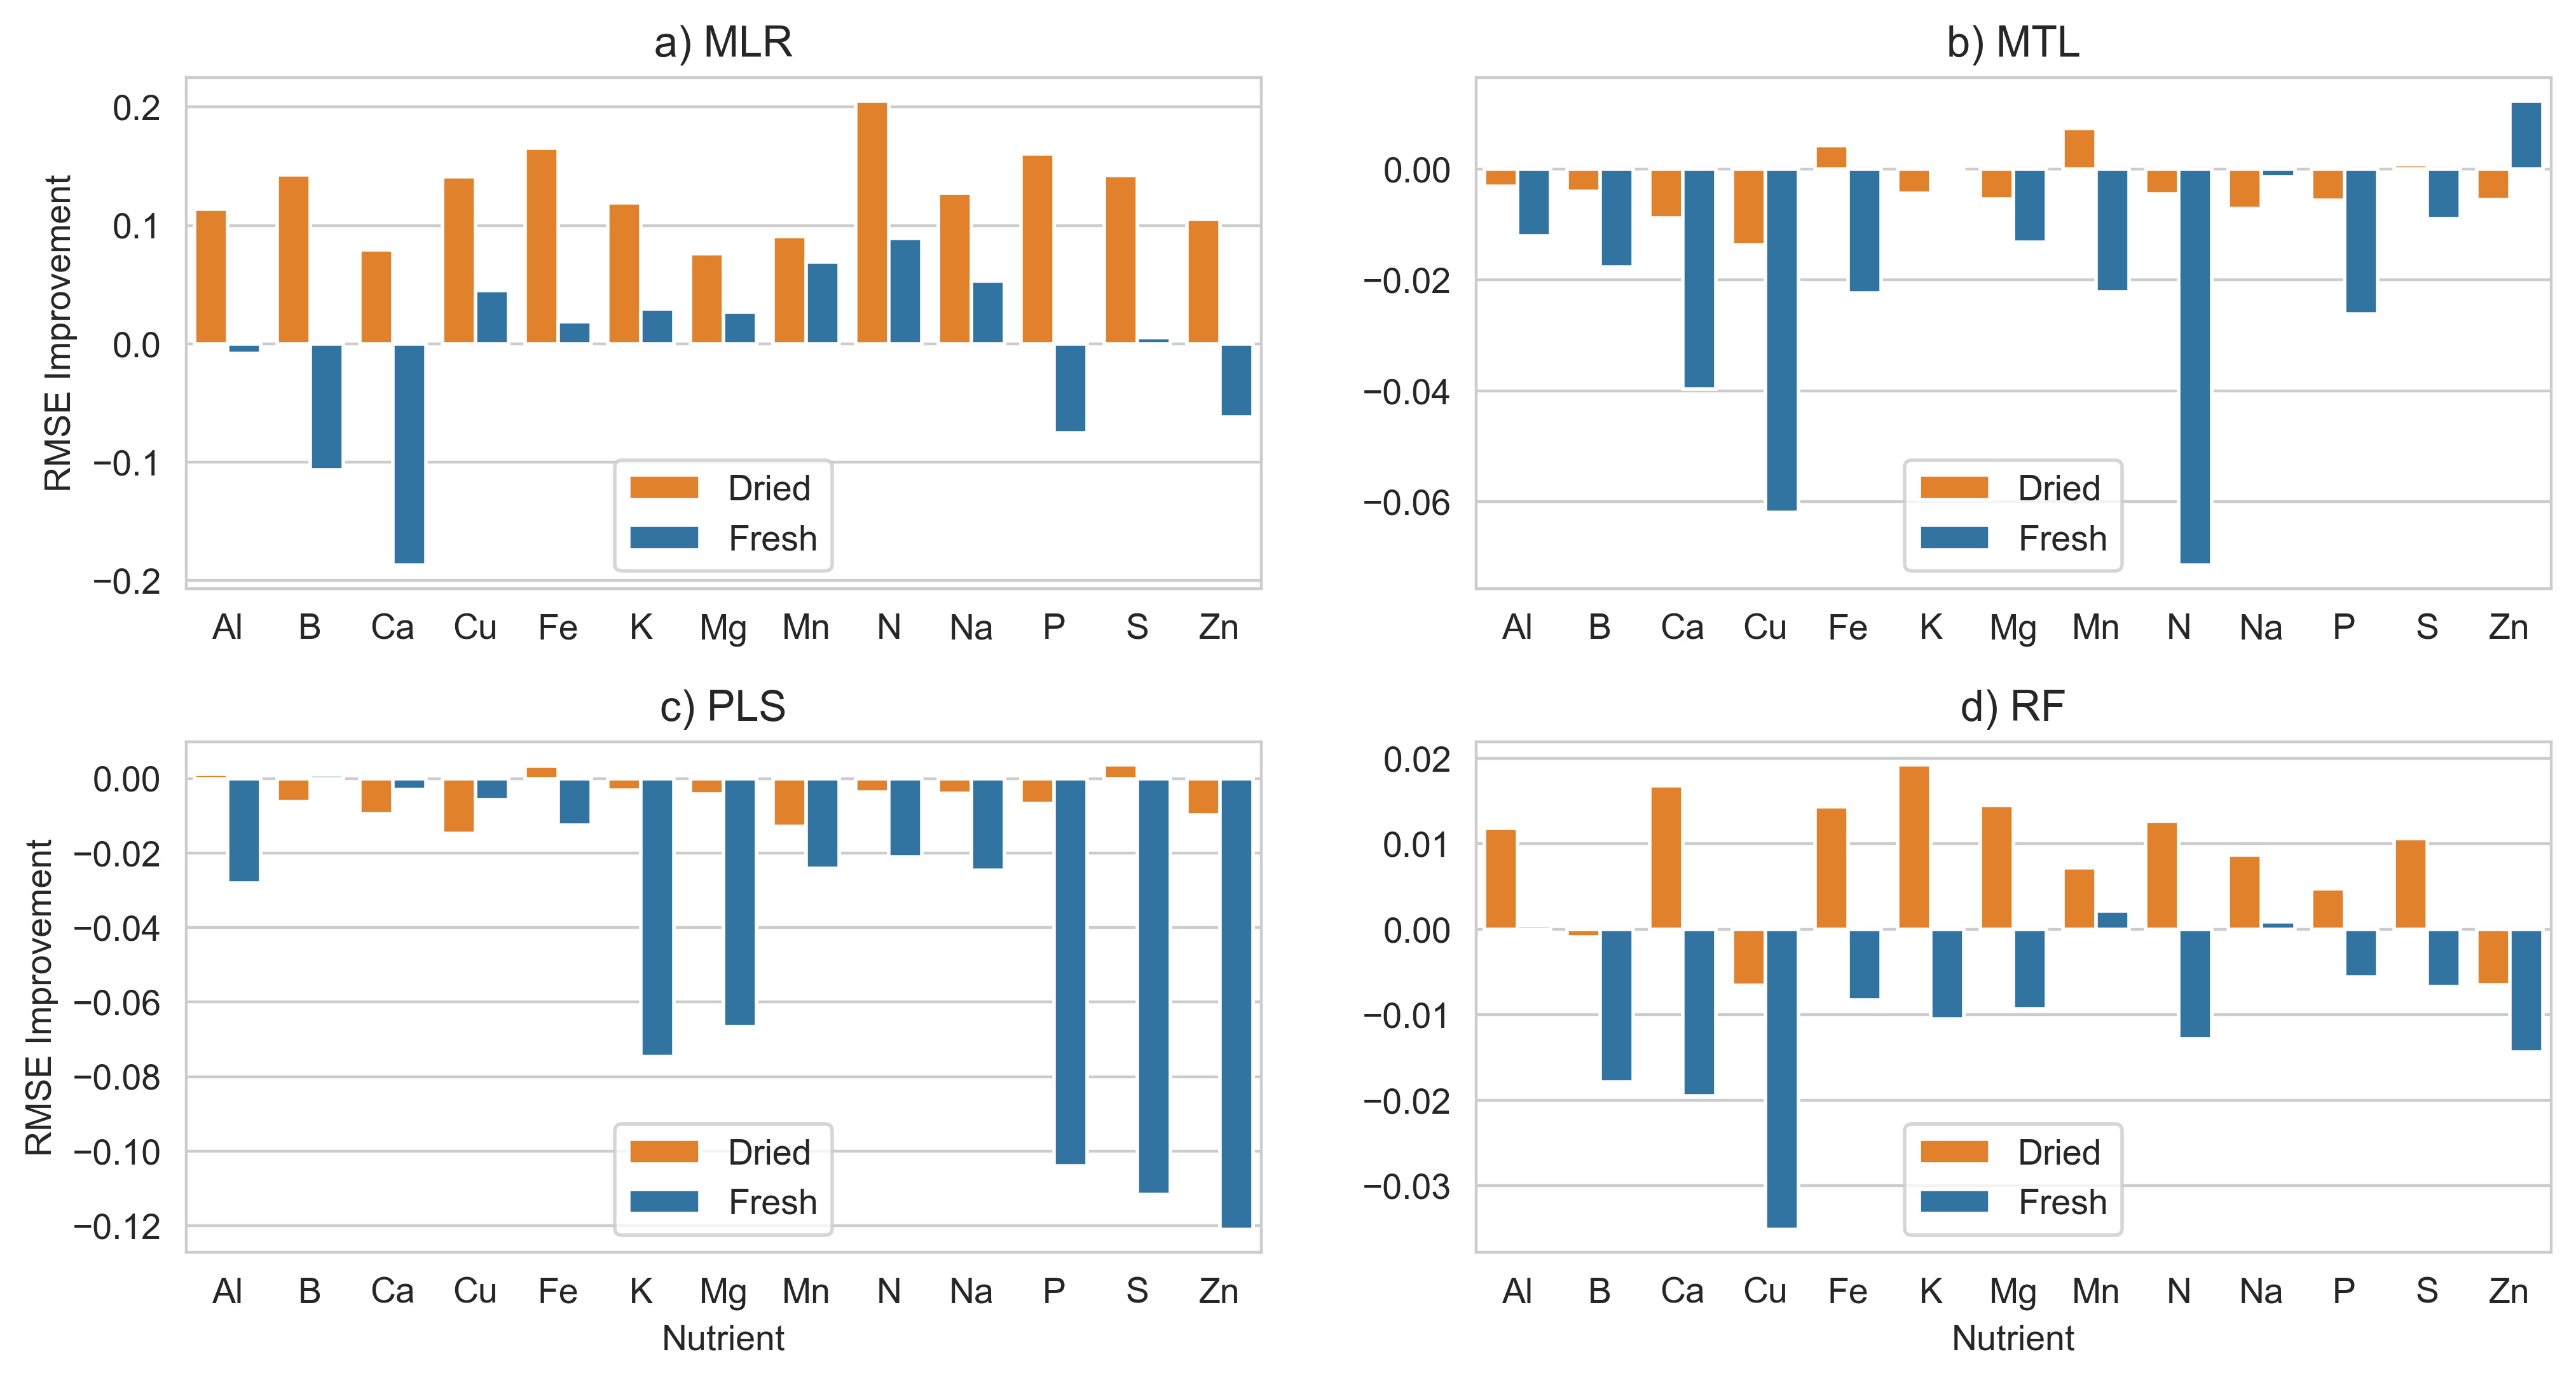
\includegraphics[width=\textwidth]{Figures/improvement_all_models.png}
    \caption{RMSE impact from ALS baseline correction with peak feature extraction for MLR, MTL, PLSR and RF.}
    \label{baseline_correction_improvement}
\end{figure*}

\begin{comment}
\begin{figure*}[!t]
    \centering
    \begin{subfigure}{\columnwidth}
        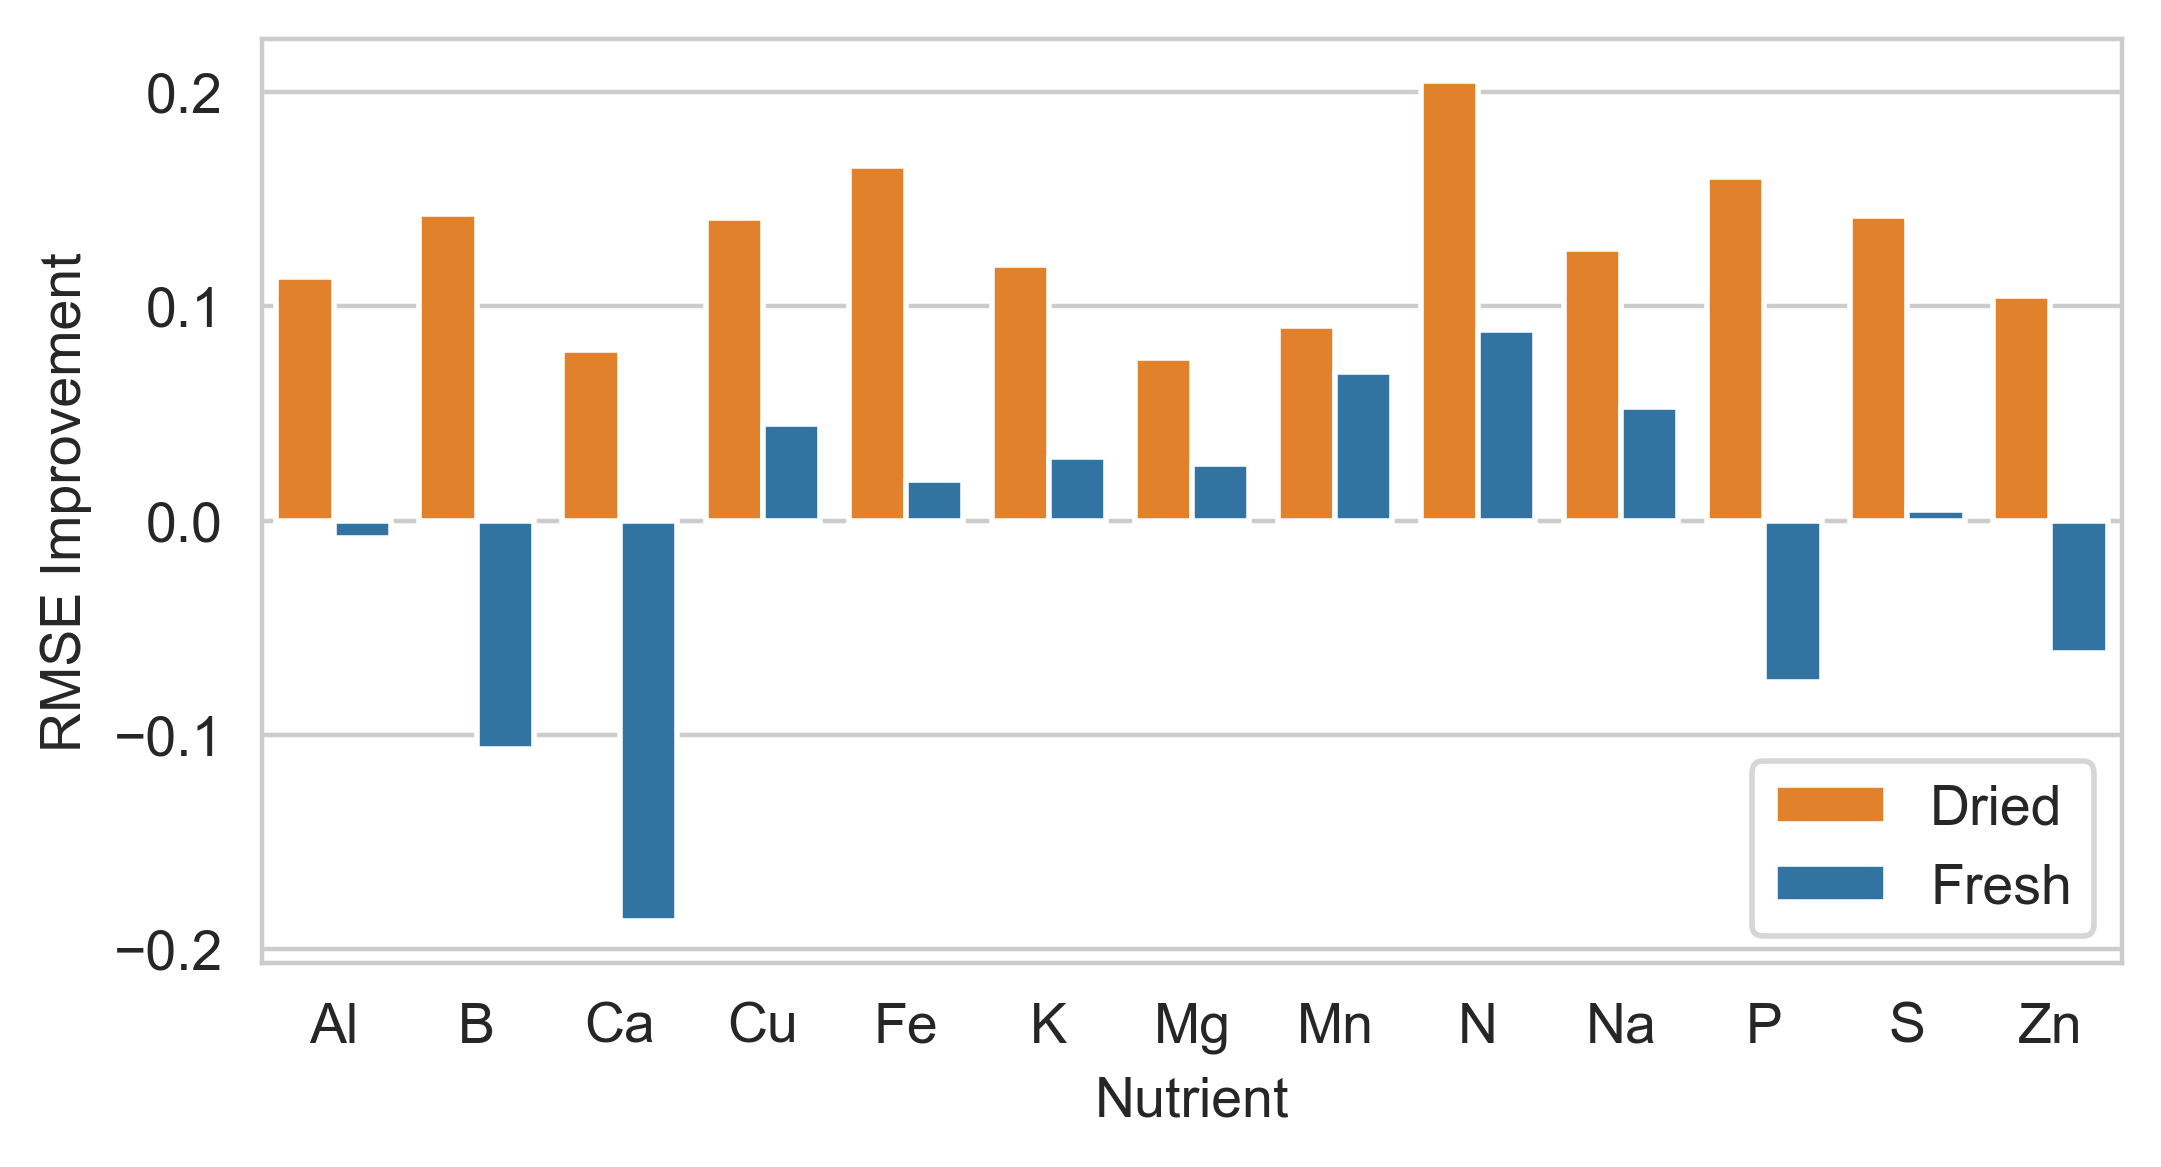
\includegraphics[width=\columnwidth]{Figures/MLR_RMSE_Baseline_Correction_Improvement.png}
        \caption{MLR improvement}
        \label{mlr_improvement}
    \end{subfigure}
    \hfil
    \begin{subfigure}{\columnwidth}
        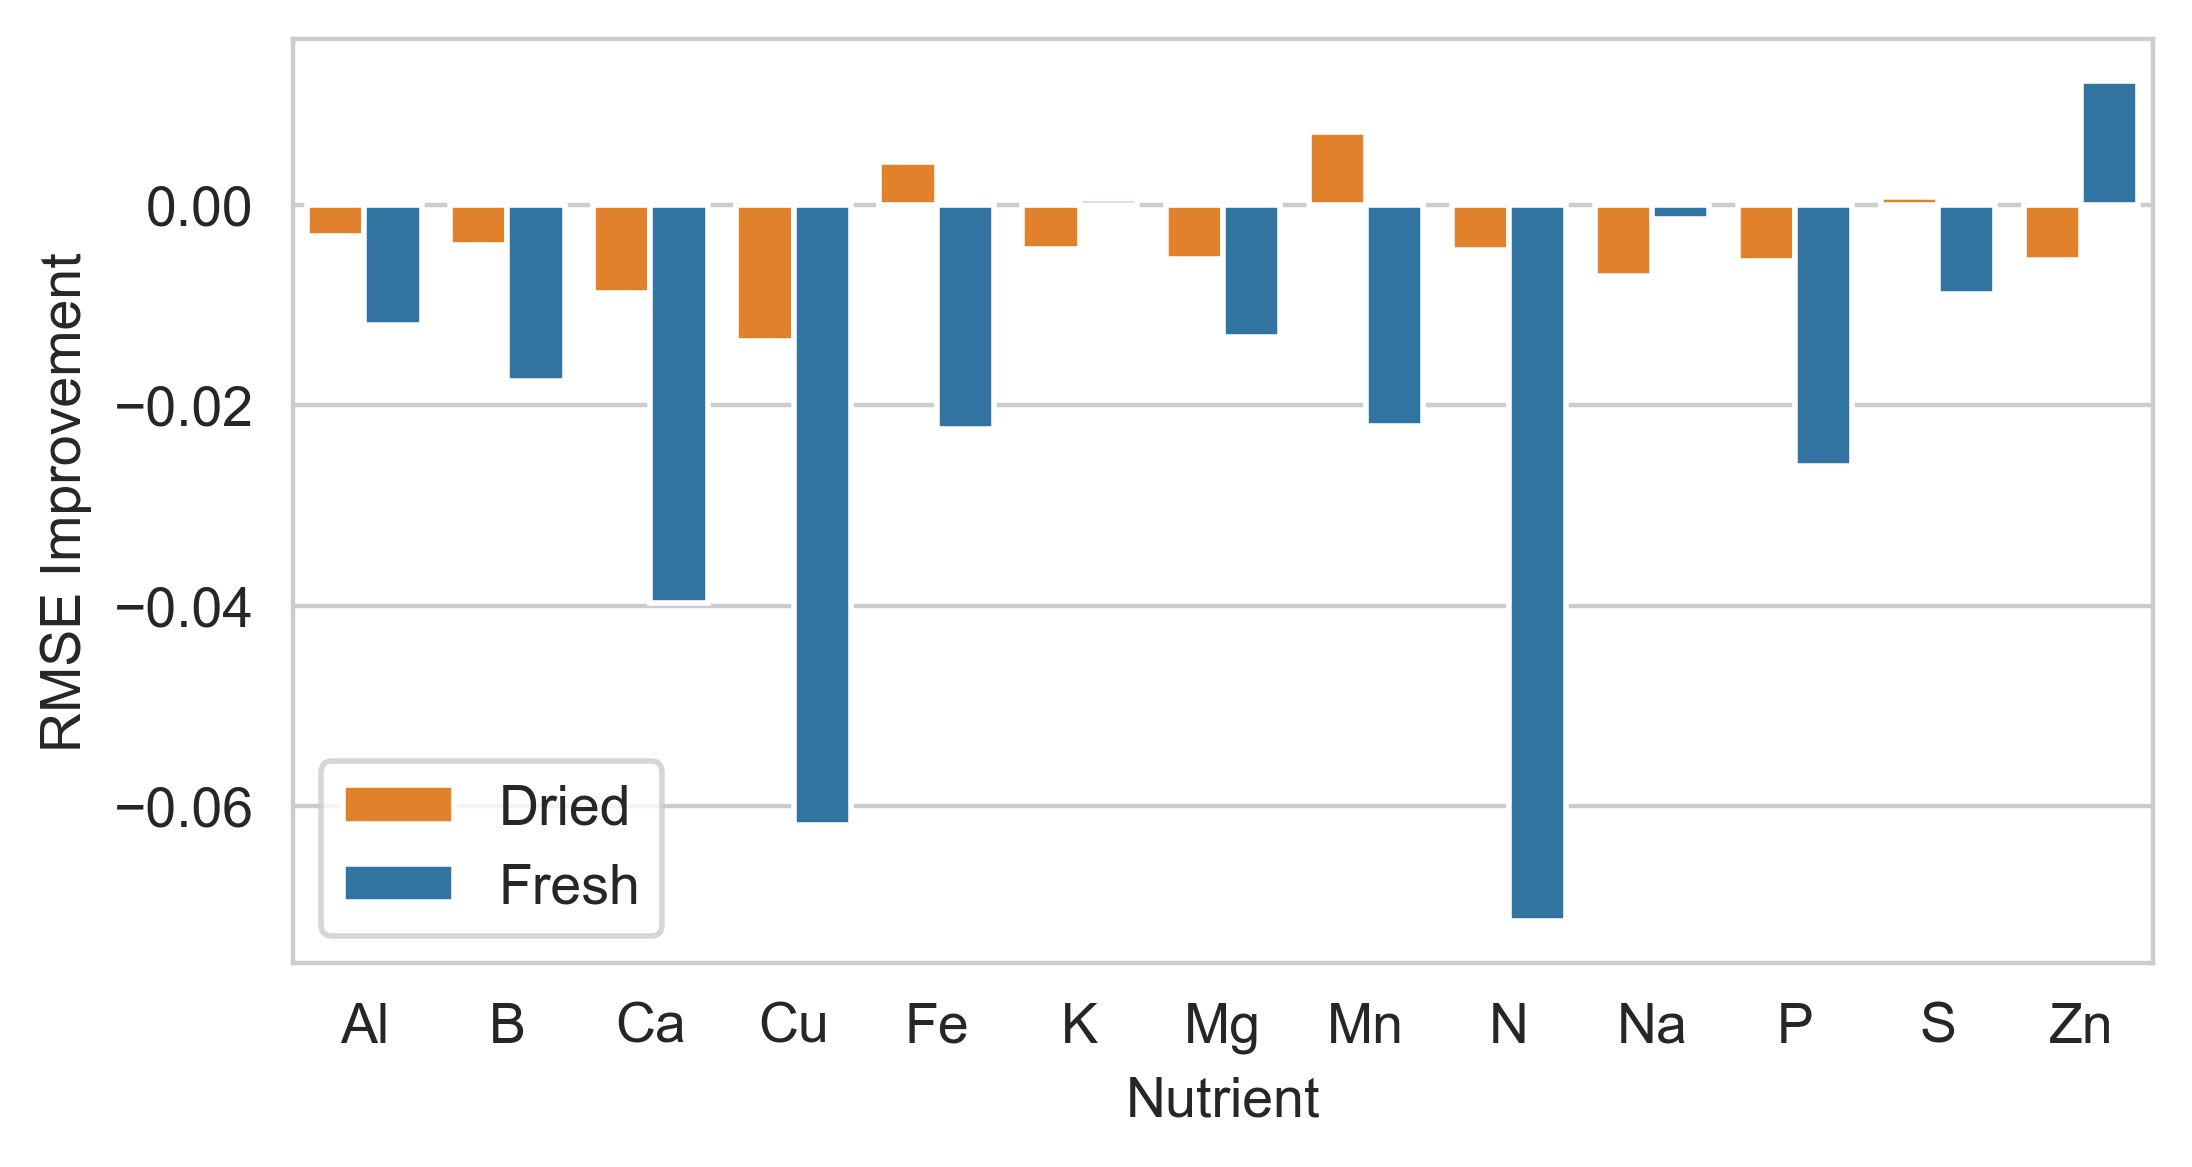
\includegraphics[width=\columnwidth]{Figures/MTL_RMSE_Baseline_Correction_Improvement.png}
        \caption{MTL improvement}
        \label{mtl_improvement}
    \end{subfigure}
    \hfil
    \begin{subfigure}{\columnwidth}
        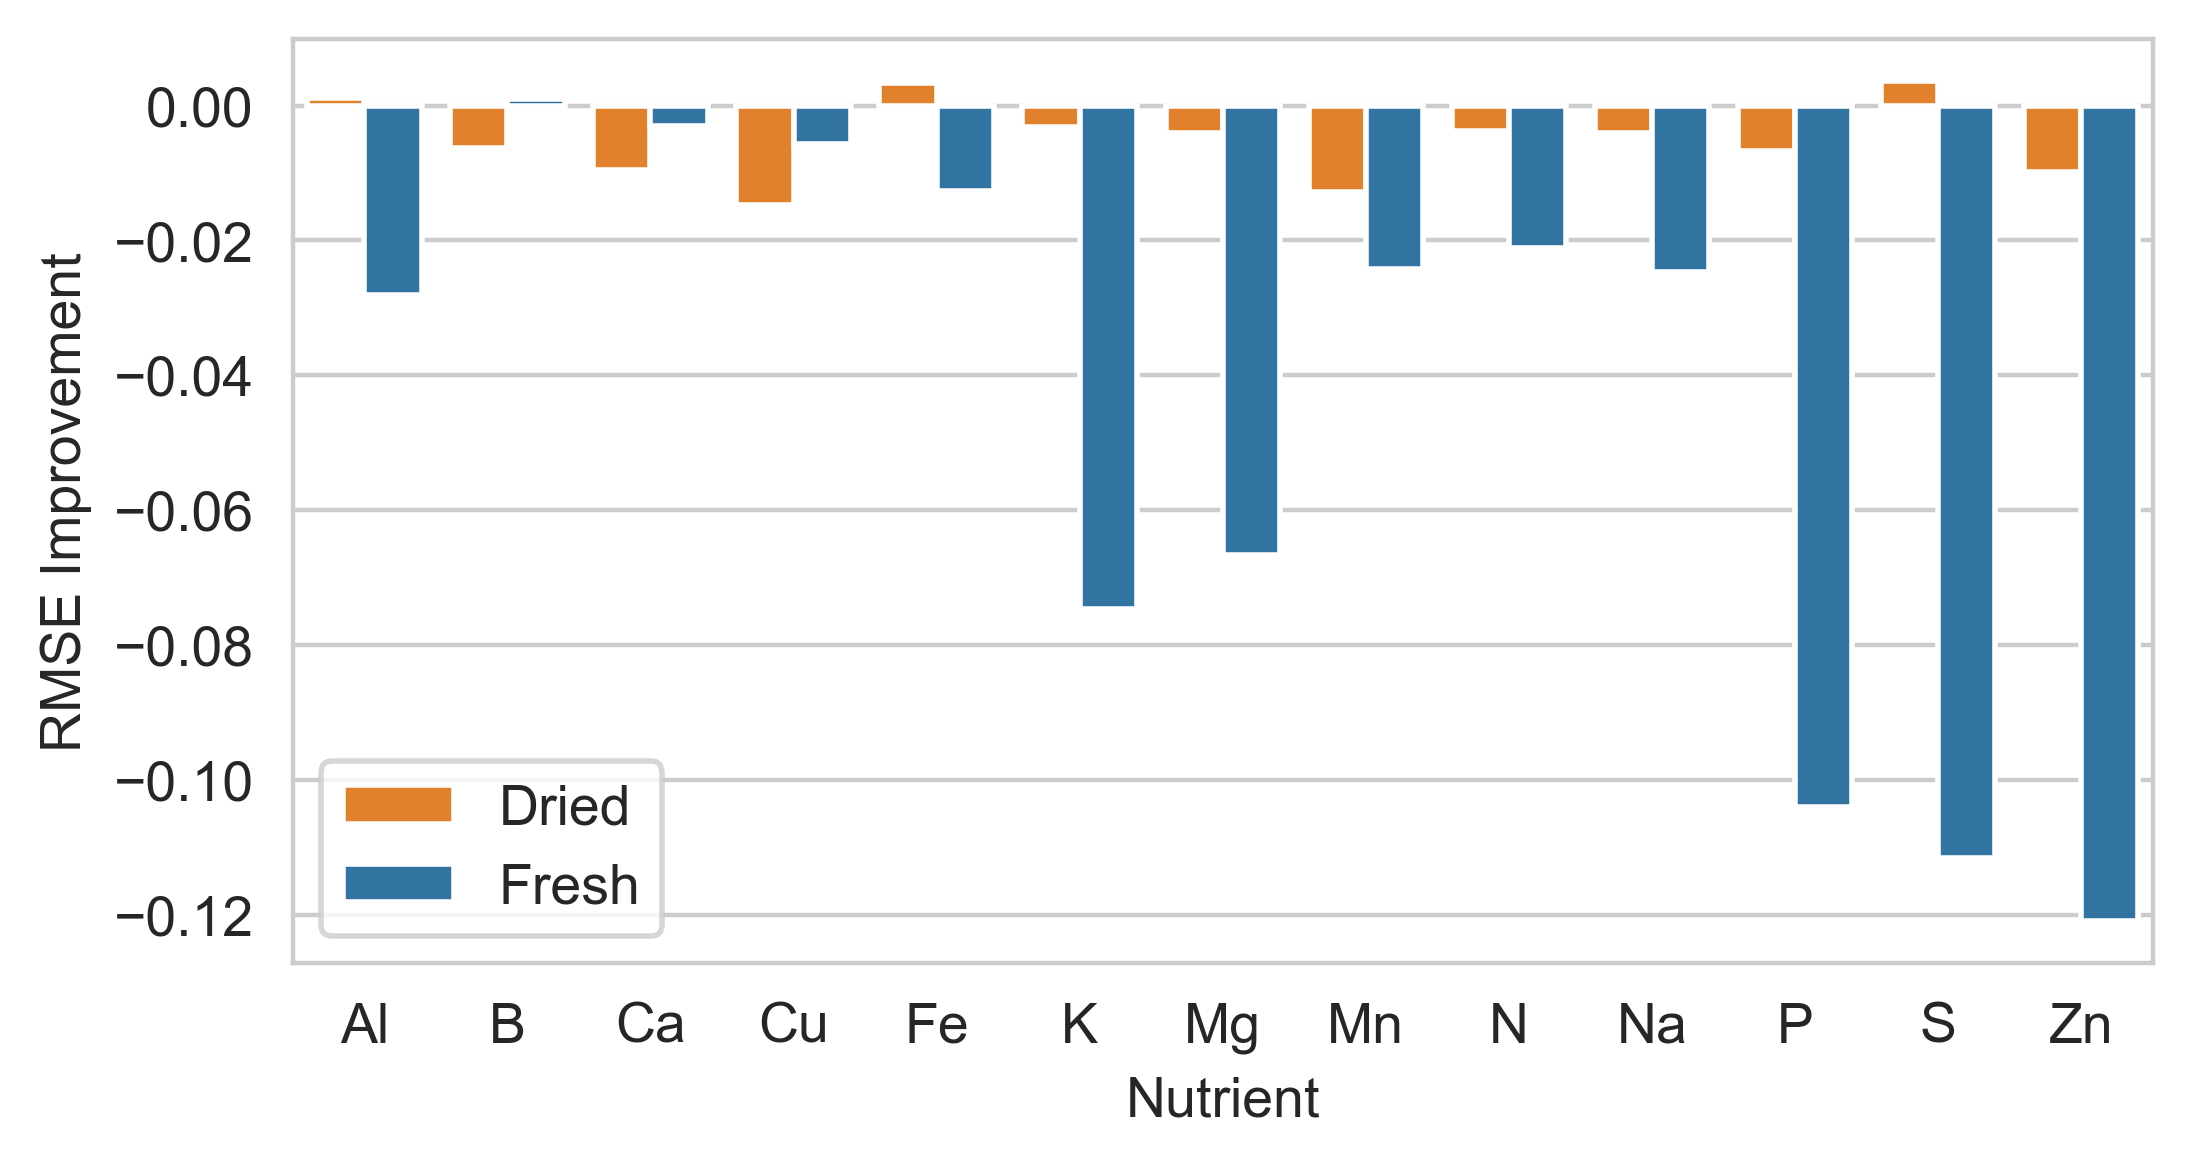
\includegraphics[width=\columnwidth]{Figures/PLS_RMSE_Baseline_Correction_Improvement.png}
        \caption{PLSR improvement}
        \label{pls_improvement}
    \end{subfigure}
    \hfil
    \begin{subfigure}{\columnwidth}
        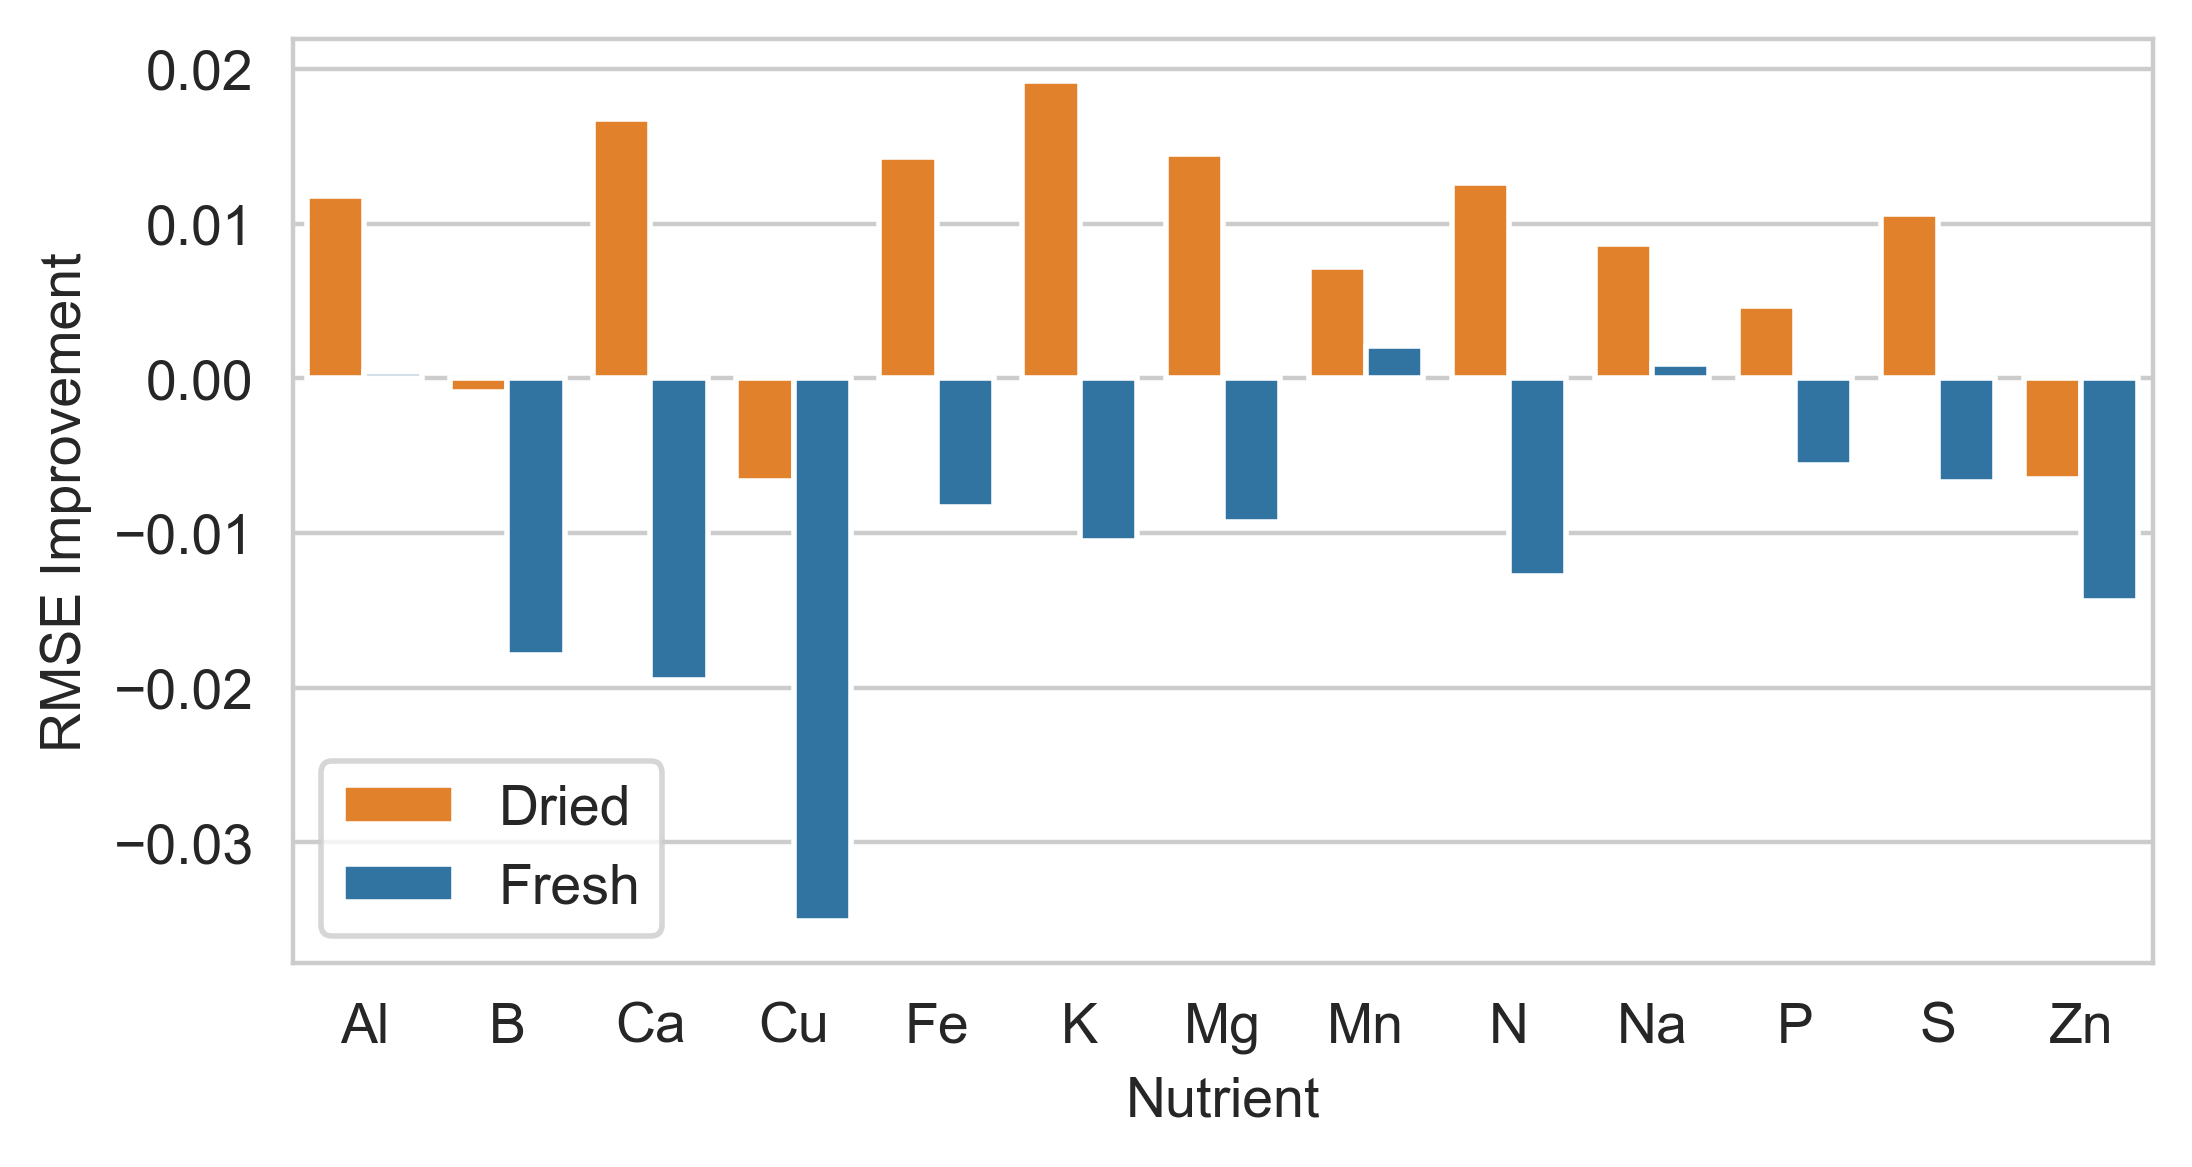
\includegraphics[width=\columnwidth]{Figures/RF_RMSE_Baseline_Correction_Improvement.png}
        \caption{RF improvement}
        \label{rf_improvement}
    \end{subfigure}
    \caption{RMSE impact from ALS baseline correction with peak feature extraction for MLR, MTL, PLSR and RF.}
    \label{baseline_correction_improvement}
\end{figure*}
\end{comment}

Results from the MVR models showed that MTEN optimised at the same hyperparameters as MTL for fresh and dried models, thus presenting the same results (Table \ref{tab:agg_results}). The $L1$ ratio of 1 meant that only $L1$ regularisation was adopted in MTEN, and optimised to a penalty term $\lambda=0.0001$, as with MTL. This penalty term means that there is minimal effect on the features. Though its uncertain why $L2$ regularisation was deferred and a minimal $L1$ penalty applied, it is expected that the applied feature selection meant the algorithm only found truly relevant features, which have a clear relationship with the target variables. Detailed results for MTEN are therefore omitted from Table \ref{tab:testresults}, which outlines all outcomes measured in $R^2$ and RMSE across the baseline model MLR against PLSR, MTL and RF on preprocessed data.

The PLSR models for fresh and dried optimised at 37 and 23 components respectively. RF optimised with 200 estimators and a maximum depth of 20 and 10 respectively.

There is a notable difference in performance between estimators for fresh and dried samples, across all models. This was anticipated based on the impact that moisture can have on infrared absorption at certain wavelengths \cite{Chon2021}, or baseline shifting due to factors such as refraction. No matter, the relationship between reflectance and moisture is complex and not necessarily linear \cite{Weidong2002}, warranting further study in this context. The RF algorithm was the least impacted and the only model achieving a positive $R^2$ score on aggregate [Table \ref{tab:agg_results}], with the least variance across nutrients. 

The results of baseline correction and peak feature extraction have noticeably diminished the predictive effectiveness of an optimised PLSR algorithm for both sample modes, particularly the fresh data. Average RMSE for fresh predictions fell from 0.1 to 0.146, particularly attributable to Mg, P, K, S, Zn which increased in error by 101\%, compared to only a 5\% increase for dried samples. PLSR appears to be affected by losing the ability to exploit correlations between the variables in the same way, given that linear relationships (on which it relies) are largely removed or distorted by the feature selection. The RF method conversely does learn relationships between these features well and can exploit non-linear relationships between variables. Comparing trained RF models on pre/post baseline corrected data showed an improvement of 8.8\% for dried samples (p value of 0.19), but an increased error of 11.1\% on average for the fresh model (p value of 0.42). From a 95\% confidence interval, this is a statistically significant result and shows a common outcome between these multi-variate models trained on pre-processed data, though at different magnitudes.

Comparing results to that of Abukmeil et al. \cite{Abukmeil2022}, they found that S had acceptable performance through Lasso MLR compared to other macronutrients as well as high $r$ (Pearson's correlation) value. While this has not been a focus of this study, our $R^2$ score for S was the lowest for nutrients in the dried testing mode, and the second poorest in the fresh testing mode ranked over all models, therefore inconsistent with the previous study based on our pipeline. However, S did show a relatively low error (RMSE=0.0842) despite its poor $R^2$ score with RF, which further reinforces the idea that this model is leveraging non-linear relationships given that the $R^2$ score reflects the linearity of the model, shown in Fig. \ref{rf_r2_rmse_comparison}. With exception to S, the figure also highlights a difference in performance for macronutrients in the dried RF model.
\begin{figure}[ht!]
\centering
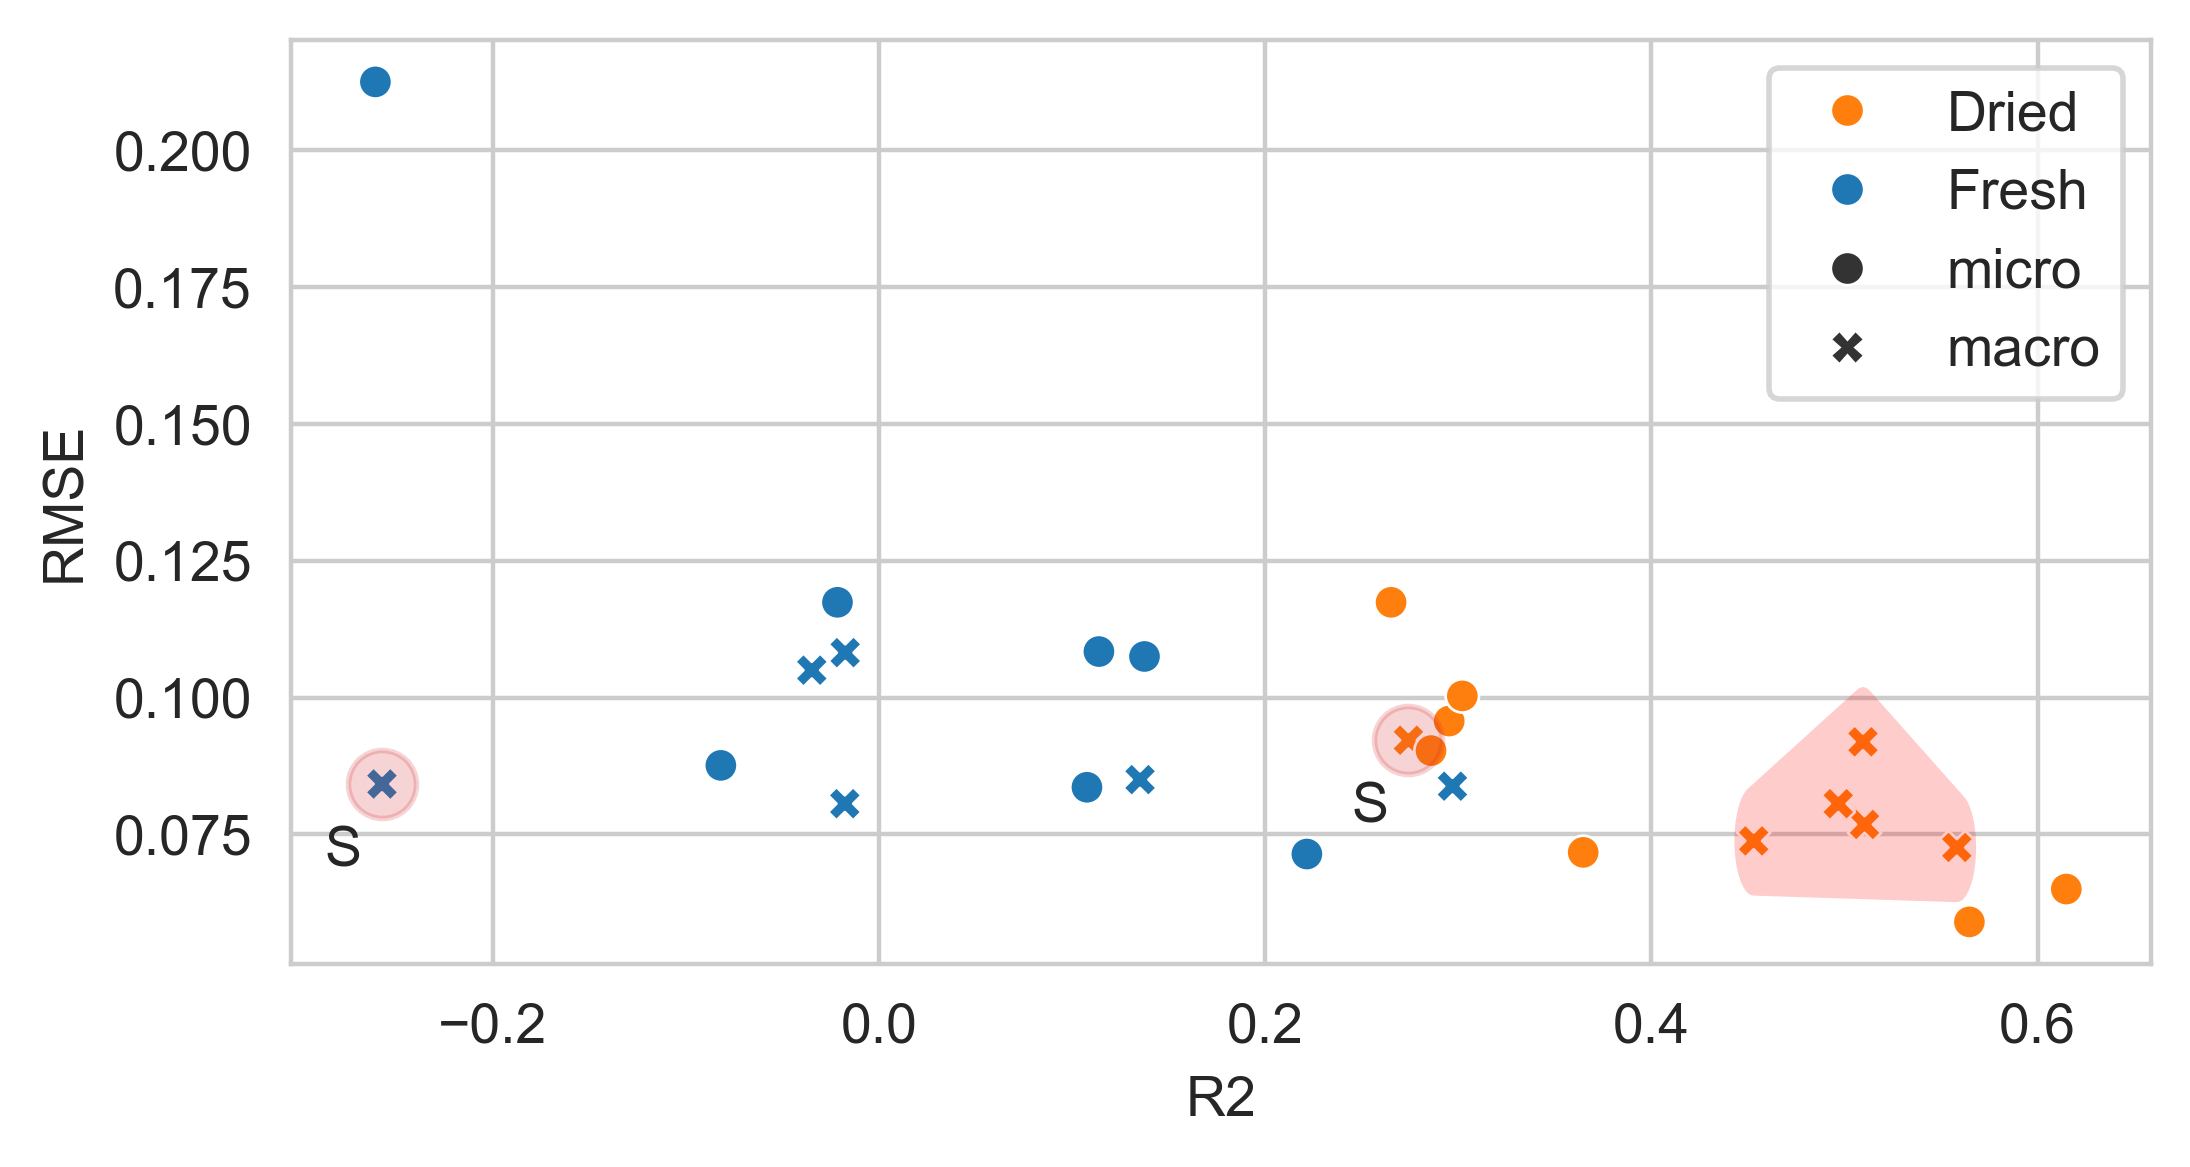
\includegraphics[width=\columnwidth]{Figures/RF_R2_RMSE.png}
\caption{$R^2$ and RMSE scores for RF, highlighting performance of S and  clustering of macro nutrient scores for dried samples.}
\label{rf_r2_rmse_comparison}
\end{figure}
Their study also showed P and K having the highest $r$ values in dried testing, and there is certain overlap with our results. K featured in the top 3 performing predictions for dried samples across all models, with a more accurate $R^2$ in the dried mode (0.57 with PLSR). With fresh, it had mediocre performance relative to other nutrients. P was the third poorest $R^2$ (-0.02, output from RF) in the fresh testing mode.

A noteworthy advantage PLSR has over RF is its efficiency in optimising its loss function over a high-dimensional dataset. PLSR can optimise over [2,45] components with 5-fold cross validation in 80 seconds, compared to training RF on a single set of hyperparameters (a maximum depth of 10, with 200 estimators) in 1hr 10min. This makes optimisation more impractical without prior DR for RF.

\begin{table}[htbp]
\caption{Aggregated metrics for each model showing optimal performance by RF, across dried and fresh sample modes.}
\begin{center}
\begin{tabular}{|c|c|c|c|c|}
\cline{2-5}
\multicolumn{1}{c|}{ } & \multicolumn{2}{|c|}{\textbf{Dried}} & \multicolumn{2}{|c|}{\textbf{Fresh}} \\
\cline{2-5}
\multicolumn{1}{c|}{ } & \textbf{$R^2$} & RMSE & \textbf{$R^2$} & RMSE \\
\hline
MLR & 0.37 & 0.0869 & -2.23 & 0.168 \\
MTL & 0.374 & 0.0868 & -0.394 & 0.1189 \\
MTEN & 0.374 & 0.0868 & -0.394 & 0.1189 \\
PLS & 0.364 & 0.0876 & -1.598 & 0.1457 \\
RF & {\color{blue}\textbf{0.423}} & {\color{blue}\textbf{0.0836}} & {\color{blue}\textbf{0.025}} & {\color{blue}\textbf{0.1027}} \\
\hline
\end{tabular}
\label{tab:agg_results}
\end{center}
\end{table}

\section{Further Work and Improvement}
Inevitably, the limited sample size of the dataset has its constraints on the ability of the trained model to generalise. Further work should be considered to extend the study with an increased sample size. This is especially applicable with fresh samples given that these were fewer and proved more difficult for the algorithms to find relationships.

Other more novel approaches, such as the use of stacked regression techniques (referenced in Section \ref{lit_review_methods}) may help to exploit different types of linear and non-linear relationships together. As the initial study of collinearity shows, some of these relationships are obvious, yet others will be less so. Exploiting the strengths of algorithms with different approaches to modelling relationship seems obvious and appears to hold benefit in alternative spectroscopy settings \cite{Cobbinah2022, Solihin2024}.

As part of the initial feasibility study, more models were assessed for their 'out-of-the-box' capability with respect to multivariate regression. Gaussian Process, Support Vector and Gradient Boosting regression model libraries assessed did not have native capability to exploit the relationships between target variables simultaneously and so were dropped. However, they all have potential and warrant more detailed assessment against the proposed pipeline given their different properties.

A final aspect that warrants further study is the ability of models to focus on particular nutrients of interest. One perspective considered as part of this study regards model training, where the importance of nutrients is weighted to focus the performance of a model biased to certain nutrients, be it through feature selection or other approach. Another perspective is the use of weighting in evaluation. Where models are assessed and compared based on an average across all nutrients, this would bias results based on chosen weights. Such approaches could help stakeholders focus treatment on nutrients they are particularly concerned with.

\section{Conclusion}
The study reveals several important observations for the domain of nutrient prediction using NIRS in potato plant leaf samples. While preprocessing reduces the number of features in a HDLSS dataset and make prediction more effective appears an obvious choice, the results of binning and PCA provide no clear benefit and (in the latter case) can cause multivariate models to overfit.

A more advanced approach utilising baseline correction (via the ALS algorithm), which serves to remove noise in the dataset prior to training, and, when combined with peak feature extraction, has proven to reduce the dimensionality of the data, highlight desired signals, and improve results. However, this improvement was not consistent across dried and fresh samples: dried samples benefitted significantly, while fresh samples did not. This highlights a key challenge in the domain — different sample modes may require tailored preprocessing pipelines to achieve reliable predictive performance. In particular, the high water content in fresh samples causes broad absorption bands and large-scale shifts in reflectance, which obscure the sharp, localised spectral features our preprocessing approach relies on to exploit. As a result, key information is lost or distorted during transformation, limiting the models’ ability to extract meaningful patterns.

The application of ALS baseline correction and peak feature extraction also had varied effects depending on the model. For models like MLR and RF, which operate on independent, well-separated features, the preprocessing steps improved accuracy by enhancing the signal-to-noise ratio and removing irrelevant spectral variation. In contrast, PLSR, which relies on capturing global linear relationships and covariation across the entire spectrum, suffered a performance drop — likely due to the removal of important latent structure during feature extraction. This suggests that while the feature selection methodology outlined in the study holds promise, its application must be carefully aligned with the modelling approach. Traditional MVR models may not be the optimal choice when key structural relationships are stripped during preprocessing.

\vspace{0.1cm}
\noindent \textbf{Project code library:} \url{https://github.com/EMATM0050-2024/dsmp-2024-groupo2}

\bibliographystyle{ieeetr}
\bibliography{references}

\clearpage
\onecolumn

\appendix

\begin{table*}[htbp]
\caption{Table of prediction metrics of fresh and dried samples for the models studied, all trained on baseline-corrected data.}
\begin{center}

\begin{tabular}{|c|c|c|c|c|c|c|c|c||c|c|c|c|c|c|c|c|}
\cline{2-17}
\multicolumn{1}{c|}{ }& \multicolumn{8}{|c||}{\textbf{Dried}}& \multicolumn{8}{|c|}{\textbf{Fresh}} \\
\cline{2-17}
\multicolumn{1}{c|}{ }& \multicolumn{2}{|c|}{\textbf{MLR}} & \multicolumn{2}{|c|}{\textbf{MTL}} & \multicolumn{2}{|c|}{\textbf{PLSR}} & \multicolumn{2}{|c||}{\textbf{RF}} & \multicolumn{2}{|c|}{\textbf{MLR}} & \multicolumn{2}{|c|}{\textbf{MTL}} & \multicolumn{2}{|c|}{\textbf{PLSR}} & \multicolumn{2}{|c|}{\textbf{RF}}  \\
\cline{2-17}
\multicolumn{1}{c|}{ } & $R^2$ & RMSE & $R^2$ & RMSE & $R^2$ & RMSE & $R^2$ & RMSE & $R^2$ & RMSE & $R^2$ & RMSE & $R^2$ & RMSE & $R^2$ & RMSE \\
\hline
\textbf{Al} & 0.29 & 0.076 & 0.45 & 0.066 & 0.48 & 0.064 & {\color{blue}\textbf{0.56}}& {\color{blue}\textbf{0.059}} & -1.38 & 0.137 & -0.16 & 0.096 & -0.62 & 0.113 & {\color{blue}\textbf{0.11}} & {\color{blue}\textbf{0.084}} \\
\textbf{B} & 0.58 & 0.068 & 0.59 & 0.067 & 0.59 & 0.067 & {\color{blue}\textbf{0.61}}& {\color{blue}\textbf{0.065}} & -3.28 & 0.241 & 0.1 & 0.11 & {\color{blue}\textbf{0.36}} & {\color{blue}\textbf{0.093}} & -0.02 & 0.117 \\
\textbf{Ca} & 0.33 & 0.09 & 0.41 & 0.084 & 0.4 & 0.085 & {\color{blue}\textbf{0.51}}& {\color{blue}\textbf{0.077}} & -8.27 & 0.314 & -0.41 & 0.123 & {\color{blue}\textbf{0.19}} & {\color{blue}\textbf{0.093}} & -0.03 & 0.105 \\
\textbf{Cu} & {\color{blue}\textbf{0.34}}& {\color{blue}\textbf{0.111}}& 0.24 & 0.119 & 0.19 & 0.123 & 0.27 & 0.117 & -0.09 & 0.197 & -0.6 & 0.239 & {\color{blue}\textbf{0.07}} & {\color{blue}\textbf{0.182}} & -0.26 & 0.213 \\
\textbf{Fe} & 0.15 & 0.105 & 0.26 & 0.098 & 0.22 & 0.101 & {\color{blue}\textbf{0.3}}& {\color{blue}\textbf{0.096}} & -0.62 & 0.147 & -0.45 & 0.139 & -0.3 & 0.132 & {\color{blue}\textbf{0.14}} & {\color{blue}\textbf{0.108}} \\
\textbf{K} & 0.5 & 0.077 & 0.53 & 0.075 & {\color{blue}\textbf{0.57}}& {\color{blue}\textbf{0.072}}& 0.56 & 0.073 & -0.58 & 0.115 & {\color{blue}\textbf{0.2}} & {\color{blue}\textbf{0.082}} & -2.06 & 0.16 & 0.14 & 0.085 \\
\textbf{Mg} & 0.47 & 0.095 & 0.49 & 0.093 & {\color{blue}\textbf{0.51}}& {\color{blue}\textbf{0.092}}& {\color{blue}\textbf{0.51}}& {\color{blue}\textbf{0.092}} & -0.2 & 0.11 & {\color{blue}\textbf{0.39}} & {\color{blue}\textbf{0.078}} & -0.87 & 0.137 & 0.3 & 0.084 \\
\textbf{Mn} & {\color{blue}\textbf{0.5}}& {\color{blue}\textbf{0.085}}& 0.46 & 0.088 & 0.3 & 0.1 & 0.3 & 0.1 & {\color{blue}\textbf{0.32}} & {\color{blue}\textbf{0.095}} & -0.14 & 0.123 & -0.22 & 0.127 & 0.11 & 0.108 \\
\textbf{N} & {\color{blue}\textbf{0.46}}& {\color{blue}\textbf{0.073}}& 0.34 & 0.081 & 0.32 & 0.082 & 0.45 & 0.074 & -0.45 & 0.096 & -2.42 & 0.148 & -0.53 & 0.099 & {\color{blue}\textbf{-0.02}} & {\color{blue}\textbf{0.081}} \\
\textbf{Na} & 0.28 & 0.076 & 0.24 & 0.079 & 0.27 & 0.077 & {\color{blue}\textbf{0.36}}& {\color{blue}\textbf{0.072}} & -0.19 & 0.089 & 0.07 & 0.078 & -0.69 & 0.105 & {\color{blue}\textbf{0.22}} & {\color{blue}\textbf{0.071}} \\
\textbf{P} & 0.42 & 0.086 & 0.4 & 0.088 & 0.4 & 0.088 & {\color{blue}\textbf{0.5}}& {\color{blue}\textbf{0.081}} & -6.34 & 0.29 & -0.81 & 0.144 & -3.35 & 0.224 & {\color{blue}\textbf{-0.02}} & {\color{blue}\textbf{0.108}} \\
\textbf{S} & 0.23 & 0.095 & 0.22 & 0.096 & {\color{blue}\textbf{0.29}}& {\color{blue}\textbf{0.091}}& 0.27 & 0.092 & -2.66 & 0.144 & -0.98 & 0.106 & -7.24 & 0.216 & {\color{blue}\textbf{-0.26}} & {\color{blue}\textbf{0.084}} \\
\textbf{Zn} & 0.25 & 0.092 & 0.23 & 0.094 & 0.19 & 0.096 & {\color{blue}\textbf{0.29}}& {\color{blue}\textbf{0.09}} & -5.26 & 0.211 & {\color{blue}\textbf{0.09}} & {\color{blue}\textbf{0.08}} & -5.54 & 0.215 & -0.08 & 0.088 \\

\hline

\end{tabular}
\label{tab:testresults}
\end{center}
\end{table*}

\end{document}
